\subsubsection{\stid{4.10} DataLib} 

\paragraph{Overview} 

Data Libraries and Services Enabling Exascale Science (DataLib). The
DataLib project encompasses multiple related activities in user-level
storage and I/O support for ECP codes on upcoming DOE platforms,
providing a number of options for effectively storing and retrieving
data and tools for assessing I/O behavior and performance.
%
The \textbf{ROMIO} and \textbf{Parallel netCDF} (PnetCDF) activities
focus on existing standards-based interfaces in broad use, assisting
in performance debugging on new platforms and augmenting existing
implementations to support new storage models (e.g., “burst
buffers”). In addition to being used directly by applications, ROMIO
and PnetCDF are also indirectly used in HDF5 and netCDF-4. Our work is
ensuring that these libraries are ready for upcoming platforms and
effective for their users (and ready as alternatives if other
libraries fall short).
%
The \textbf{Darshan} I/O characterization toolset is an instrumentation tool
deployed at facilities to capture information on I/O behavior of
applications running at scale on production systems. It has become
popular at many DOE facilities and is usually “on by default”. Darshan
data dramatically accelerates root cause analysis of performance
problems for applications and can also (in some cases) assist in
correctness debugging. Our work in this project focuses on extending
Darshan to new interfaces and ensuring readiness on upcoming
platforms.
%
The \textbf{Mochi} and \textbf{Mercury} software tools are building blocks for
user-level distributed HPC services. They address issues of
performance, programmability, and portability in this key facet of
data service development. Mercury is being used by Intel in the
development of their DAOS storage service and in other data service
activities, while within ECP the HXHIM and UnifyCR projects also have
plans to leverage these tools. In addition to working with these
stakeholders and ensuring performance and correctness on upcoming
platforms, we are also working with ECP application teams to customize
data services for their needs (e.g., memoization, ML model management
during learning).

\paragraph{Key Challenges}

Each of these subprojects has its own set of challenges. Libraries
such as ROMIO and PnetCDF have numerous users from over a decade of
production use, yet significant changes are needed to address the
scale, heterogeneity, and latency requirements of upcoming
applications. New algorithms and methods of storing data are required.
%
For Darshan, the challenge is to operate in a transparent manner in
the face of continuing change in build environments, to grow in
functionality to cover new interfaces while remaining ``lean'' from a
resource utilization perspective, and to interoperate with other tools
that use similar methods to hook into applications.
%
Mochi and Mercury are new tools, so the challenge in the context of
these tools is to find users, adapt and improve to better support
those users, and gain a foothold in the science community.

\paragraph{Solution Strategy}

\emph{Transparently refactoring application I/O.}
Collective I/O is an important optimization in codes where phases of
I/O are naturally identifiable: individual I/O operations from
application processes are transparently refactored (i.e., without
application code changes) to achieve the same goals at lower cost. We
will improve collective I/O techniques for Exascale through tighter
integration with I/O forwarding layers, topology awareness, and
employing collective approaches in higher-level libraries where
additional information is available.

\emph{Intermediate storage and alternative data organizations.}
Nonvolatile memory (NVM) or
solid-state disk (SSD) integrated into platforms provides a pool of
fast storage where data can be stored temporarily or staged for
writing to an external store (e.g., parallel file system). Recognizing
that this data is transient, alternative organizations (e.g.,
provide higher performance.

\emph{Capturing and reconstructing I/O behavior.}
Darshan characterizes fully the POSIX and MPI-IO layers and captures
some statistics for HDF5 and PnetCDF. We will improve our coverage of
HDF5, PnetCDF, and ADIOS to better enable understanding of these
codes. We will reach out to other library teams to consider
characterization of them as well (e.g., SCR, FTI, PIO, SILO).

\emph{Mercury porting and support for relevant platforms.}
Mercury is an RPC/bulk data communication library for use in HPC
services and co-developed by the HDF Group. We will work with system
vendors to enable efficient Mercury communication on the platforms of
interest (e.g., UCX/PAMI on IBM).

\emph{Data service co-design with application teams.}
A number of candidate ECP applications have data service needs (e.g.,
material property databases, producer-consumer data pipelines,
multi-scale/physics simulation coupling, multi-modal data organization
and indexing). We will identify application teams with data service
requirements that are particularly ill-suited to solution by vendor
offerings (e.g., parallel file systems, standard burst buffers,
cloud-based databases) and co-design, develop, and evolve specialized
services based on our components to meet their specific requirements
for ECP.

\paragraph{Recent Progress}

\emph{Darshan.}
Darshan has won a 2018 R\&D 100 Award. The award is given by R\&D magazine
to the 100 top new technologies for the year. The Darshan software
package enables researchers to investigate and tune the I/O behavior of
complex high-performance computing (HPC) applications. A key feature of
the package is its ability to run on some of the largest systems in the
world, including Crays, IBM Blue Gene systems and Linux clusters. 

We've begun designing automatic tracing in Darshan (STDM12-13), starting
with an analysis of use cases provided by a number of stakeholders.


\emph{Mochi and Mercury.}
Nightly tests are now running on Aires, InfiniBand, and OmniPath networks
(STDM12-7). See below for more information on STDM12-7.

\emph{PnetCDF.}
Figure~\ref{fig:pnetcdf} illustrates a refactoring of the PnetCDF
library to include a dispatch layer. The dispatch layer provides a
mechanism for implementing multiple back-ends under the standard
API. This functionality is being used to enable writing in a log
format for intermediate data and access of data in the netCDF-4 format
(stored in HDF5 files).

The PnetCDF Burst Buffer capabilities have been tested, and results were
published at the PDSW workshop in conjunction with SC18 (STDM12-10).
ADIOS and netCDF-4 read capabilities have been implemented in PnetCDF,
and testing of ADIOS read capabilities under PnetCDF (STDM12-11) is
underway.
%
We continue to make improvements in support of E3SM workloads.

\emph{ROMIO.}
Integration of pipelined I/O functionality into ROMIO (STDM12-9) is complete,
specifically into the Lustre driver. We continue to improve the LogFS
ROMIO back-end.

\emph{ParSplice.}
Work with ParSplice is complete for now (STDM12-21). Specialized segment
store attains similar performance as a tightly integrated solution for
current problem sizes. As the application team scales up, we expect
the scalability of the segment store to provide a performance benefit,
but this is TBD.

\emph{Portage/JALI}. Examining Portage/JALI as next candidate for service
specialization (STDM12-21).

\begin{figure}[htb]
        \centering
        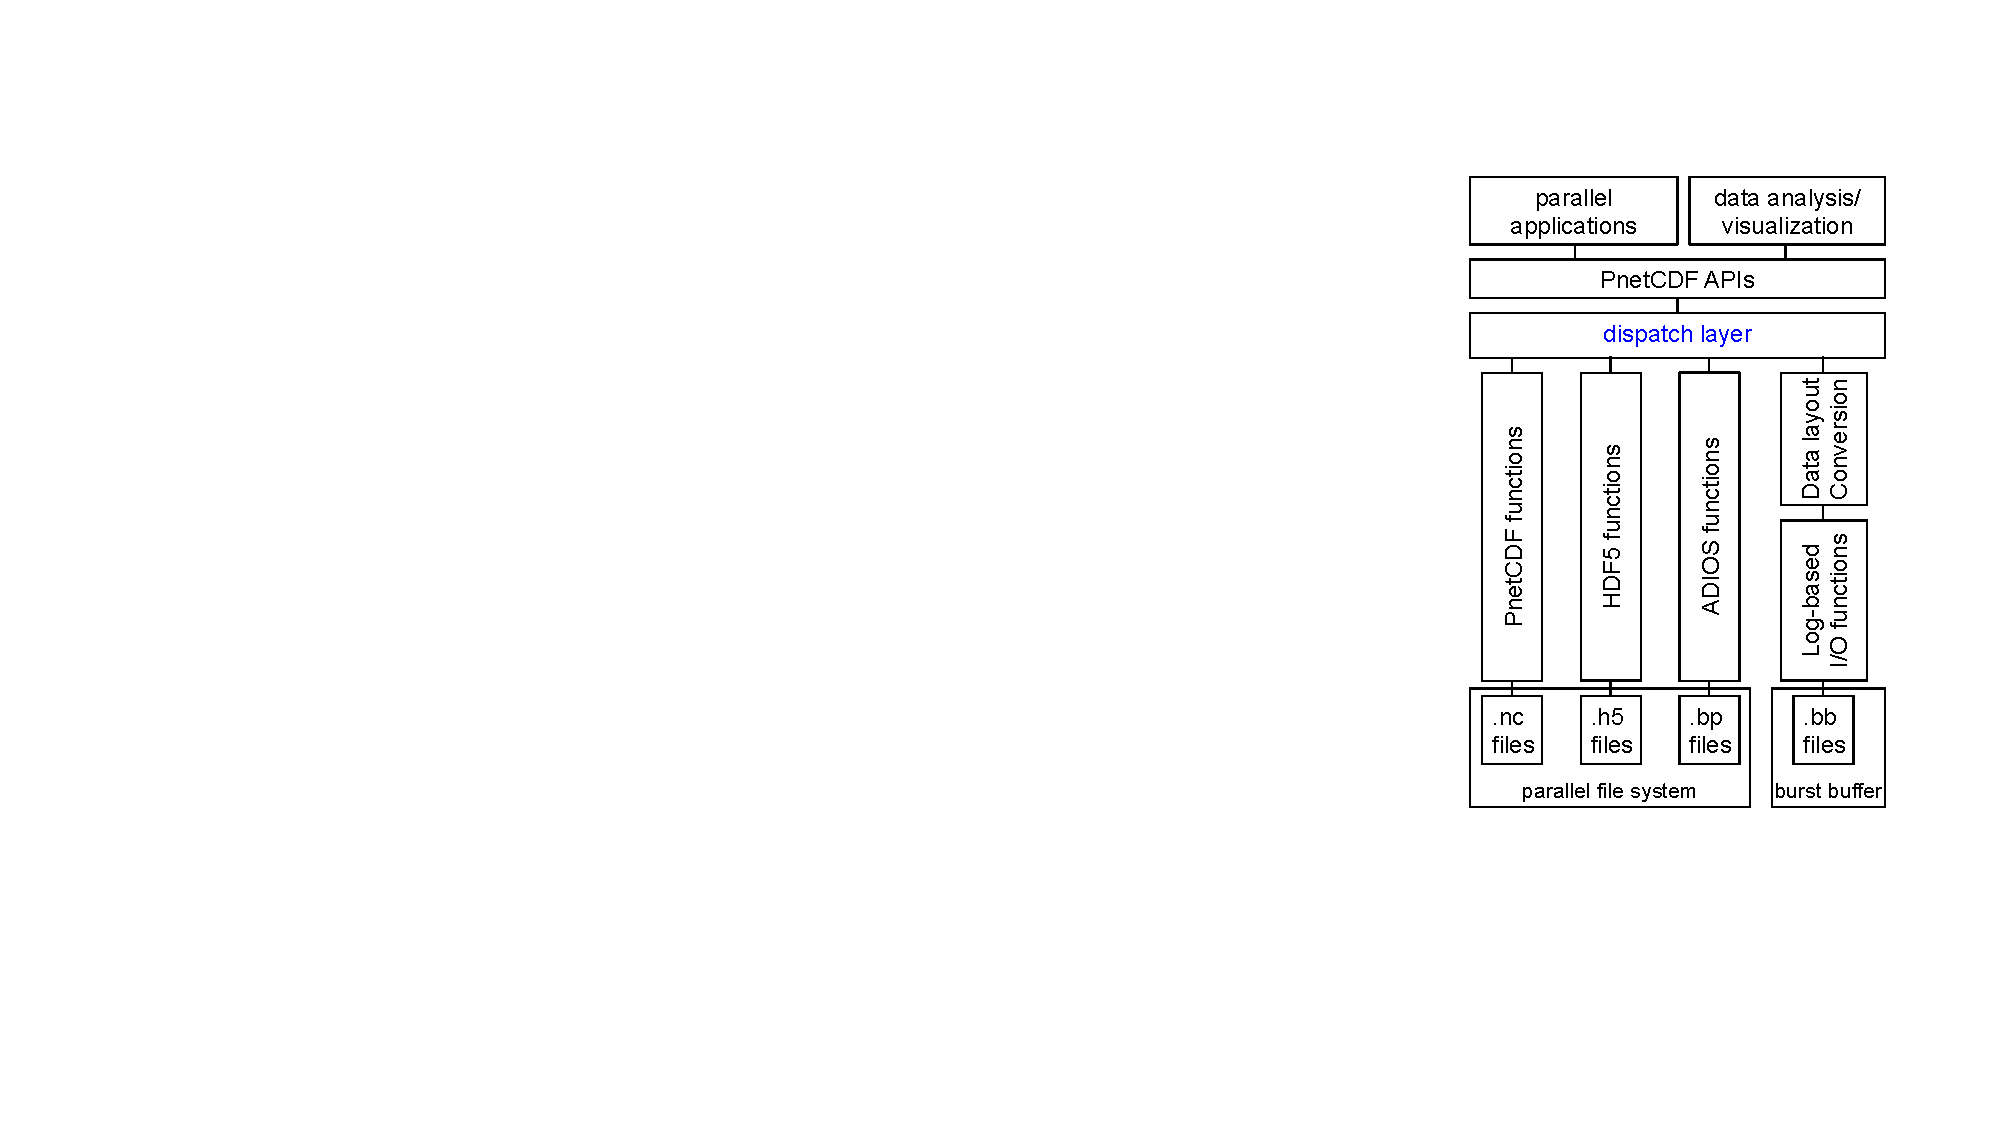
\includegraphics[height=2.5in]{projects/2.3.4-DataViz/2.3.4.10-DataLib/pnetcdf-figure.pdf}
        \caption{\label{fig:pnetcdf} The new PnetCDF dispatch layer provides flexibility to target different back-end formats and devices under the PnetCDF API used by many existing applications.
        }
\end{figure}

\paragraph{Next Steps}
Closing on the end of our first three year project period, we are focusing
on (a) wrapping up software releases of Darshan, PnetCDF, and Mercury
suite (STDM12-13, STDM12-11, and STDM12-12); (b) adding new optimized
collective I/O capabilities in ROMIO (STDM12-14); (c) completing automatic
triggering of tracing in Darshan (STDM12-13); and (d) investigating
additional use cases of specialized services in ECP applications
(STDM12-21). 

